\documentclass[reqno]{amsart}
\usepackage[utf8]{inputenc}
\usepackage[margin=1in]{geometry}
\usepackage[usenames, dvipsnames]{xcolor}
\usepackage{graphicx}
\usepackage{mathtools}
\usepackage{amssymb}
\usepackage{amsthm}
\usepackage{fancyhdr}
\usepackage{adforn}
\usepackage{xparse}
\usepackage{tikz}
\usetikzlibrary{fadings}
%\usetikzlibrary{matrix, positioning, calc}
% Additional math macros that I want in both my notes and my psets
\usepackage[sc, noBBpl]{mathpazo}
\usepackage{mathrsfs}
\usepackage[T1]{fontenc}
\usepackage{calligra}
\usepackage{microtype}
\usepackage[all]{xy}
\usepackage{slashed}
\newcommand{\A}{\mathbb A}
\newcommand{\cat}{\mathsf}
\newcommand{\sC}{\cat C}
\newcommand{\sD}{\cat D}
\newcommand{\sS}{\cat S}
\newcommand{\sA}{\mathscr A}
\newcommand{\sF}{\mathscr F}
\newcommand{\sG}{\mathscr G}
\renewcommand{\P}{\mathbb P}
\newcommand{\cO}{\mathscr O}
\newcommand{\sI}{\mathscr I}
\DeclareMathOperator{\coker}{coker}
\renewcommand{\Im}{\operatorname{Im}}
\newcommand{\pt}{\mathrm{pt}}
\DeclareMathOperator{\Hom}{Hom}
\newcommand{\op}{^{\mathsf{op}}}
\newcommand{\Id}{\mathrm{Id}}
\DeclareMathOperator{\Mat}{Mat}
\newcommand{\m}{\mathfrak m}
%\newcommand{\p}{\mathfrak p}
\newcommand{\q}{\mathfrak q}
\DeclareMathOperator{\MSpec}{MSpec}
\DeclareMathOperator{\Spec}{Spec}
\newcommand{\Top}{\cat{Top}}
\newcommand{\Ring}{\cat{Ring}}
\newcommand{\Mod}{\cat{Mod}}
\DeclareMathOperator{\res}{res}
\newcommand{\Alg}{\cat{Alg}}
\newcommand{\Fun}{\cat{Fun}}
\newcommand{\AffSch}{\cat{AffSch}}
\newcommand{\Ab}{\cat{Ab}}
\DeclareMathOperator{\bl}{--}
\DeclareMathOperator{\Free}{Free}
\DeclareMathOperator{\For}{For}
\newcommand{\Set}{\cat{Set}}
\newcommand{\LocRing}{\cat{LocRing}}
\newcommand{\Grp}{\cat{Grp}}
\newcommand{\Sch}{\cat{Sch}}
\newcommand{\inHom}{\operatorname{\underline{\Hom}}}
\DeclareMathOperator{\Frac}{Frac}
\DeclareMathOperator{\Gal}{Gal}
\DeclareMathOperator{\Nil}{Nil}
\newcommand{\pre}{\sC^{\text{pre}}}
\newcommand{\sh}{_{\text{sh}}}
\newcommand{\G}{\mathbb G}
\DeclareMathOperator{\Proj}{Proj}
\newcommand{\sM}{\mathscr M}
\newcommand{\sV}{\mathscr V}
\newcommand{\fU}{\mathfrak U}
\newcommand{\GL}{\mathrm{GL}}
\DeclareMathOperator{\Sym}{Sym}
% http://tex.stackexchange.com/questions/141434/how-to-type-sheaf-hom
\DeclareMathOperator{\shom}{\mathscr{H}\text{\kern -4pt {\calligra\large om}}\,}
\newcommand{\sL}{\mathscr L}
\DeclareMathOperator{\QC}{QC}
\DeclareMathOperator{\Supp}{Supp}
\newcommand{\sN}{\mathscr N}
\DeclareMathOperator{\Ann}{Ann}
\DeclareMathOperator{\Der}{Der}
\newcommand{\ctcpx}[1]{(#1)^{\text{der}}}
\newcommand{\Dist}{\mathsf{Dist}}
\newcommand{\shdi}{\operatorname{Sh}_{\Dist}}
\DeclareMathOperator{\Sh}{Sh}
\newcommand{\shz}{\mathsf{Sh}_{\text{\rm Zar}}}
\DeclareMathOperator{\Gr}{Gr}
% Source: http://tug.org/pipermail/xy-pic/2001-July/000015.html
\newcommand{\pullbackcorner}[1][dr]{\save*!/#1+1.2pc/#1:(1,-1)@^{|-}\restore}
\newcommand{\pushoutcorner}[1][dr]{\save*!/#1-1.2pc/#1:(-1,1)@^{|-}\restore}
\newcommand{\TDel}{\mathrm{2\Delta}}
\DeclareMathOperator{\Bl}{B\ell}
\newcommand{\cR}{\mathcal R}
\newcommand{\cL}{\mathcal L}
\newcommand{\cH}{\mathcal H}
\newcommand{\refR}{\reflectbox{\(\cR\)}}

\renewcommand{\a}{\alpha}
\renewcommand{\b}{\beta}
%\newcommand{\e}{\epsilon}
\renewcommand{\l}{\lambda}
\renewcommand{\L}{\Lambda}
\newcommand{\g}{\gamma}
\newcommand{\s}{\sigma}
\newcommand{\z}{\zeta}
\newcommand{\RR}{\mathbb{R}}
\newcommand{\NN}{\mathbb{N}}
\newcommand{\QQ}{\mathbb{Q}}
\newcommand{\ZZ}{\mathbb{Z}}
\newcommand{\CC}{\mathbb{C}}
\newcommand{\cC}{\mathcal{C}}
\newcommand{\f}{\frac}
\newcommand{\p}{\partial}
\renewcommand{\P}[3][]{\f{\partial^{#1} #2}{\partial #3 ^{#1}}}
%\newcommand{\avg}[1]{\langle #1 \rangle}
\newcommand{\avg}[1]{\left< #1 \right>}
\newcommand{\?}{\overset{?}{=}}
\newcommand{\Int}{\int_{-\infty}^\infty}
\newcommand{\ket}[1]{\left| #1 \right>} % for Dirac bras
\newcommand{\bra}[1]{\left< #1 \right|} % for Dirac kets
\newcommand{\braket}[2]{\left< #1 \vphantom{#2} \right|
 \left. #2 \vphantom{#1} \right>} % for Dirac brackets
\newcommand{\pv}{\vec{p}}

\newcommand{\grad}[1]{\gv{\nabla} #1} % for gradient
\let\divsymb=\div % rename builtin command \div to \divsymb
\renewcommand{\div}[1]{\gv{\nabla} \cdot #1} % for divergence
\newcommand{\curl}[1]{\gv{\nabla} \times #1} % for curl
\renewcommand{\labelenumi}{(\alph{enumi})}
\let\vaccent=\v % rename builtin command \v{} to \vaccent{}
\renewcommand{\v}[1]{\ensuremath{\mathbf{#1}}}
\newcommand{\uv}[1]{\ensuremath{\mathbf{\hat{#1}}}} % for unit vector
\newcommand{\gv}[1]{\ensuremath{\mbox{\boldmath$ #1 $}}} 
% for vectors of Greek letters
\usepackage{hyperref}
\usepackage{siunitx}

%\usepackage[compat=1.1.0]{tikz-feynman}

% TODO fiddle with colors
\definecolor{newblue}{HTML}{1F98A6}
\definecolor{newred}{HTML}{D95448}
\definecolor{neworange}{HTML}{F29441}
\hypersetup{
	colorlinks,
	linkcolor=newred,
	citecolor=neworange,
	urlcolor=newblue!80!black,
}
\usepackage[all]{hypcap}
\pagestyle{plain}
\setcounter{tocdepth}{1}


\usepackage{titlesec}
\titleformat{\section}[frame]
  {\normalfont}
  {\filright
   \footnotesize
   \enspace Lecture \arabic{section}.\enspace}
  {8pt}
  {\Large\bfseries\filcenter}
\usepackage[dotinlabels]{titletoc}
\titlecontents{section}[1.5em]{}{\contentslabel{2.3em}}{\hspace*{-2.3em}}{\hfill\contentspage}

\renewcommand{\sectionmark}[1]{\markleft\thesection. #1}

\fancyhf{}
\fancyhead[RO,LE]{\small\thepage}
\fancyhead[LO]{\small\slshape\nouppercase{\rightmark}}
\fancyhead[RE]{\small\slshape Advanced Quantum Field Theory Lecture Notes}
\setlength{\headheight}{11.0pt}
\pagestyle{fancy}

\numberwithin{equation}{section}
\newcommand{\orbreak}{
\begin{center}
	\adforn{17}\;\(\cdot\)\;\adforn{18}
	\vspace{0.2cm}
\end{center}
}

\renewcommand{\labelitemi}{\(\circ\)}

% I wanted to allow one to reference parts of a thm/cor/etc. and have it print the thm number too, e.g. 29.2(1),
% but this isn't working right now. Probably the best way to do this would be to play around with enumitem to
% define a new enumerate-like counter and then just use that directly instead of enumerate in comp.

% This feels really wobbly, but so far it's working
\NewDocumentEnvironment{comp}{mm}{%
	\csname #1\endcsname\hfill
	\csname #2\endcsname
}{
	\csname end#2\endcsname
	\csname end#1\endcsname
}

% usage:
% \shortexact[f][g]{A}{B}{C},
%
%			 f    g
% for 0 -> A -> B -> C -> 0,
\DeclareDocumentCommand{\shortexact}{O{} O{} mmmm}{
\xymatrix{
	0\ar[r] & #3\ar[r]^-{#1} & #4\ar[r]^-{#2} & #5\ar[r] & 0#6
}}
% exactly the same, but for 0 -> A -> B -> C
\DeclareDocumentCommand{\leftexact}{O{} O{} mmmm}{
\xymatrix{
	0\ar[r] & #3\ar[r]^-{#1} & #4\ar[r]^-{#2} & #5 #6
}}
% ... and the same, for A -> B -> C -> 0
\DeclareDocumentCommand{\rightexact}{O{} O{} mmmm}{
\xymatrix{
	#3\ar[r]^-{#1} & #4\ar[r]^-{#2} & #5\ar[r] & 0#6
}}



% usage:
% X\dblarrow[r] & Y
%   f
% X => Y
%   g
\DeclareDocumentCommand{\dblarrow}{O{} O{} O{}}{
	\ar@<0.4ex>[#1]^-{#2}\ar@<-0.4ex>[#1]_-{#3}
}
% Note: it would be a useful exercise to figure out how to define this so it can be used as
% \dblarrow[r]^f_g

\everyentry={\displaystyle}

\newcommand{\N}{\mathbb N}
\newcommand{\Z}{\mathbb Z}
\newcommand{\Q}{\mathbb Q}
\newcommand{\R}{\mathbb R}
\newcommand{\C}{\mathbb C}
\newcommand{\F}{\mathbb F}
\newcommand{\vp}{\varphi}
\newcommand{\term}{\emph}
\renewcommand{\vec}[1]{\boldsymbol{\mathbf{#1}}}
\DeclarePairedDelimiter\paren{(}{)}
%\DeclarePairedDelimiter\ang{\langle}{\rangle}
\DeclarePairedDelimiter\abs{\lvert}{\rvert}
\DeclarePairedDelimiter\norm{\lVert}{\rVert}
\DeclarePairedDelimiter\bkt{[}{]}
\DeclarePairedDelimiter\set{\{}{\}}
% Swap paren* and paren, etc., so that the normal version resizes by default.
% Meanwhile, one can use \paren*[\Big]{...} to customize the size easily.
% It would be interesting to wrap this up into a custom \definedelimiter command...
\makeatletter
	\let\oldparen\paren
	\def\paren{\@ifstar{\oldparen}{\oldparen*}}
	\let\oldbkt\bkt
	\def\bkt{\@ifstar{\oldbkt}{\oldbkt*}}
\makeatother
\newcommand{\e}{\varepsilon}
\def\qedsymbol{{\small{\ensuremath{\boxtimes}}}}
\newcommand{\inj}{\hookrightarrow}
\newcommand{\surj}{\twoheadrightarrow}
\DeclareMathOperator{\id}{id}
\newcommand{\ud}{\,\mathrm{d}}
\renewcommand{\d}{\mathrm d}
\newcommand{\dfr}[2]{\frac{\mathrm d #1}{\mathrm d #2}}
\newcommand{\pfr}[2]{\frac{\partial #1}{\partial #2}}

%\catcode`\"=13
%\newcommand{"}[1]{^{(#1)}}
\newtheorem{thm}[equation]{Theorem}
\newtheorem*{thm*}{Theorem}
\newtheorem{lem}[equation]{Lemma}
\newtheorem*{lem*}{Lemma}
\newtheorem{cor}[equation]{Corollary}
\newtheorem{prop}[equation]{Proposition}
\newtheorem{obs}[equation]{Observation}
\theoremstyle{definition}
\newtheorem{ex}[equation]{Exercise}
\newtheorem{exm}[equation]{Example}
\newtheorem{defn}[equation]{Definition}
\newtheorem*{claim}{Claim}
\theoremstyle{remark}
\newtheorem*{rem}{Remark}
\newtheorem*{fct}{Fact}
\newtheorem*{note}{Note}

\begin{document}
\title{General Relativity}
\author{Ian Lim\\ Michaelmas 2018}
\maketitle
{\small\noindent These notes were taken for the \textit{General Relativity} course taught by Malcolm Perry at the University of Cambridge as part of the Mathematical Tripos Part III in Michaelmas Term 2018. I live-\TeX ed them using TeXworks, and as such there may be typos; please send questions, comments, complaints, and corrections to 
\href{mailto:itel2@cam.ac.uk?subject=GR\%20Lecture\%20Notes}{\texttt{itel2@cam.ac.uk}}.\\
Many thanks to Arun Debray for the {\LaTeX} template for these lecture notes: as of the time of writing, you can find him at \url{https://web.ma.utexas.edu/users/a.debray/}.}

\tableofcontents
\clearpage
\section{Friday, October 5, 2018}
	Unlike in previous years, this course is intended to be a stand-alone course on general relativity, building up the mathematical formalism needed to construct the full theory and explore some examples of interesting spacetime metrics. It is linked to the Black Holes course taught in Lent term, which I will also be writing notes for.

Some recommended course materials and readings include the following:
\begin{itemize}
\item Sean Carroll, Spacetime and Geometry
\item Misner, Thorne, and Wheeler, Gravitation
\item Wald, General Relativity
\item Zee, Einstein Gravity in a Nutshell
\item Hawking and Ellis, ``The Large Scale Structure of Spacetime''
\end{itemize}

In Minkowski\footnote{I've heard some USAmericans pronounce this ``min-cow-ski.'' In German, it is ``min-koff-ski.''} spacetime (flat space) we specify points in spacetime by spatial coordinates in $\RR^3$, i.e. the Cartesian coordinates $(x,y,z)$, plus a time coordinate $t$. The line element (spacetime separation) is given by the metric
$$ds^2=-dt^2+dx^2+dy^2+dz^2.$$
$ds$ is the proper distance between $x$ and $x+dx$, $y$ and $y+dy$, $z$ and $z+dz$, and $t$ and $t+dt$. (As is typical in relativity, we work in units where $c=1$. Note that the metric sign convention here is flipped from my QFT notes, which uses the ``mostly minus'' convention-- this is arbitrary and so long as one is consistent it makes no difference.) Using the Einstein summation convention, the metric is usually written more compactly as $$ds^2=\eta_{\alpha\beta}x^\alpha x^\beta,$$ with $\eta_{\alpha\beta}$ the Minkowski space metric.

Let's recall from special relativity that we call separations with $ds^2>0$ ``spacelike,'' with $ds^2<0$ ``timelike,'' and $ds^2=0$ null (or occasionally lightlike).
\begin{defn}
The \term{chronological future} of a point $p$ is the set of all points that can be reached from $p$ along future directed timelike lines, and we call this $I^+(p)$. It is the interior of the future-directed light cone. Conversely we have the chronological past of $p$, $I^-(p)$, which is the interior of the past-directed light cone. We also have the \term{causal future} of $p$, which is the set of all points that can be reached from $p$ along future-directed timelike \emph{or} null lines, and we call this $J^+(p)$. Similarly we have the causal past, $J^-(p)$. Thus $J$ is the closure of $I$ and is the interior \emph{plus} the light cone itself.
\end{defn}

\begin{figure}
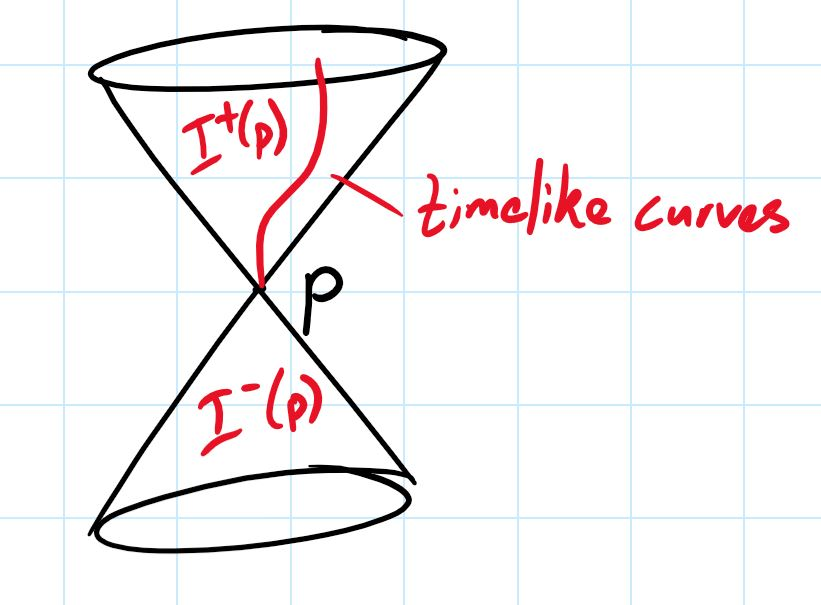
\includegraphics{2018/10/20181005_img1}
\caption{An illustration of the light cones from a point $p$, plus the chronological future $I^+$ and chronological past $I^-$. Also depicted in red is a timelike curve (e.g. a possible particle trajectory in spacetime).}
\end{figure}

Let $x^a(\tau)$ be a curve in spacetime.\footnote{Evidently we are not using the convention that Greek indices range from $0$ to $3$ and Latin indices range from $1$ to $3$. I have copied the lecturer's convention here, but may change to more traditional notation if it becomes relevant.} Then the tangent vector to the curve is $u^a=\frac{dx^a}{d\tau}$. For timelike curves, $u^a u^b \eta_{ab}=-1 \iff \tau$ is the proper time along the curve.
\footnote{The property that $U^\alpha U^\beta \eta_{\alpha\beta}=-1$ is easy to prove. See the Special Relativity catch-up sheet found \href{http://www.maths.cam.ac.uk/sites/www.maths.cam.ac.uk/files/grspecialrelativity.pdf}{here} for some nice exercises in SR: this is exercise 3. Assuming the result of exercise 2 which states that the four-velocity of a massive particle is $U^\mu=\gamma(1,v^i)$, we then have $U\cdot U =\gamma^2(-1+v^2)=\frac{v^2-1}{1-v^2}=-1$. Since this is a fully contracted expression (no indices floating around), it is true in all frames.}
We also know that $\int_p^q d\tau = \Delta \tau$, which just says that the integral of $d\tau$ along a curve from $p$ to $q$ yields the proper time interval, what a clock actually measures.

We also remark that Minkowski space has some very nice symmetries. Since $x,y,$ and $z$ do not appear explicitly in the metric, our spacetime is invariant under translations. It is also invariant under rotations in $\RR^3$. It would be nice to extend rotations to include the time coordinate $t$ as well-- this is exactly what a Lorentz transformation does.

Lorentz transformations in general involve time-- they are defined by the matrices $\Lambda$ which satisfy
$$\Lambda^T \eta \Lambda= \eta,$$
i.e. they preserve the inner product $\eta$ in Minkowski space, forming the group $O(3,1)$. Lorentz transformations consist of rotations in $\RR^3$ and boosts. This is equivalent to the defining property of rotation matrices $R$ that $R^T \delta R=\delta$, meaning that rotation matrices preserve the standard Euclidean inner product in $\RR^3$ and form the group $O(3)$.\footnote{Strictly, $O(3)$ also includes reflections-- for matrices which preserve both orientation and the inner product, we must also require that $\det R=+1$, defining the group $SO(3)$. We'll see a similar caveat with the Lorentz group in just a second.}
Written explicitly, the Lorentz boost in the $x$-direction to a frame moving with velocity $v$ is
\begin{eqnarray*}
t\to t'&=&\frac{t-vx}{\sqrt{1-v^2}}\\
x\to x'&=&\frac{x-vt}{\sqrt{1-v^2}}\\
y\to y'&=&y\\
z\to z'&=&z
\end{eqnarray*}
We may also write it in matrix notation,
$${\Lambda^a}_b =
\begin{pmatrix}
\gamma&-\gamma v &0 & 0\\
-\gamma v & \gamma & 0 & 0\\
0&0&1&0\\
0&0&0&1
\end{pmatrix}$$
where $\gamma$ is defined in the usual way by $\gamma \equiv \frac{1}{\sqrt{1-v^2}}$.

Rather than constructing the (in general complicated) Lorentz boost in an arbitrary direction, it is often more convenient to rotate one's frame of reference in $\RR^3$ so the boost is in the new $x$-direction, perform the Lorentz boost, and then transform back:
$$R^T \Lambda R= \Lambda_R,$$
where $\Lambda_R$ is a new Lorentz transformation.\footnote{It's easy to check that $\Lambda_R$ really is a Lorentz transformation-- just observe that rotations alone are a subset of Lorentz transformations, since they preserve the inner product on $\RR^3$ and do not affect the time coordinate. In the language of group theory, rotations form an $SO(3)$ subgroup of the full Lorentz group $O(3,1)$-- see Definition \ref{lorentzgroup}. Therefore any combination of rotations and Lorentz boosts will form another valid Lorentz transformation by the group closure property.}

\begin{defn}\label{lorentzgroup}
The Lorentz transformations taken together form the \term{Lorentz group}. It satisfies the group axioms of identity, unique inverses (since $\det\Lambda \neq 0$), associativity (from associativity of matrix multiplication), and closure (see footnote for proof).\footnote{More precisely, we know that the determinant is nonzero since $-1=\det{\eta}=\det(\Lambda^T\eta\Lambda)=\det(\Lambda^T)\det(\eta)\det(\Lambda)=(-1)\det(\Lambda)^2\implies \det(\Lambda)=\pm 1 \neq 0$. To prove closure, suppose $\Lambda_1,\Lambda_2$ are Lorentz transformations. The product $\Lambda_1\Lambda_2$ then satisfies $(\Lambda_1\Lambda_2)^T \eta(\Lambda_1\Lambda_2)= \Lambda_2^T \Lambda_1^T \eta\Lambda_1 \Lambda_2 = \Lambda_2^T \eta \Lambda_2 = \eta$, so $\Lambda_1\Lambda_2$ is also a Lorentz transformation.}
\end{defn}

$\Lambda$ can include reflections in time or space. To avoid such complications, we sometimes refer to the \term{proper orthochronous Lorentz group,} i.e. to exclude space and time reversals, but often we are more careless and simply call it the Lorentz group.
\begin{defn}
The \term{Poincar\'e group} is then the semidirect product of Lorentz transformations and translations. This is the group of symmetries of Minkowski space.
\end{defn}
We have translations defined as
$$x^a\to {x^a}'=x^a+\Delta x^a$$
and also Lorentz transformations, with the property
$${(\Lambda^T)_a}^c \eta_{cd} {\Lambda^d}_b=\eta_{ab}.$$


\begin{defn}
We also have \term{contravariant vectors} (indices up) written $u^a$ and their corresponding \term{covariant} vectors (indices down) $$u_a\equiv\eta_{ab}u^b,$$ where we have used the metric to lower an index. These are sometimes equivalently called simply vectors and covectors. We can also raise indices using the inverse metric $\eta^{ab}$ (defined by $\eta^{ab}\eta_{bc}=\delta^a_c$). Thus
$$u^b=\eta^{ba}u_a.$$
\end{defn}

We define the Lorentz transformation of a contravariant vector as
$u^a\to {u^a}' = {\Lambda^a}_b u^b.$  For instance, $x^a$ is an example of a contravariant vector.

\begin{defn}
A \term{scalar} is an object which is invariant under a Lorentz transformation. We saw that a covariant vector transforms with right multiplication by the Lorentz transformation, whereas a contravariant vector transforms by left multiplication. 

More generally, a \term{tensor of type $(r,s)$} transforms with $r$ copies of the Lorentz transformation on the $r$ up indices and $s$ copies of the Lorentz transformation on the $s$ down indices, 
\begin{equation}
{T^{\mu_1 \mu_2\ldots \mu_r}}_{\nu_1 \nu_2 \ldots \nu_s} \to {T^{\alpha_1 \alpha_2\ldots \alpha_r}}_{\beta_1 \beta_2 \ldots \beta_s}=\Lambda^{\alpha_1}_{\mu_1} \ldots \Lambda^{\alpha_r}_{\mu_r} {T^{\mu_1 \mu_2\ldots \mu_r}}_{\nu_1 \nu_2 \ldots \nu_s} \Lambda^{\nu_1}_{\beta_1}\ldots \Lambda^{\nu_s}_{\beta_s}
\end{equation}

By this definition, a scalar may be thought of as a type $(0,0)$ tensor, a contravariant vector a type $(1,0)$ tensor, and a covariant vector a type $(0,1)$ tensor.
\end{defn}

\section{Monday, October 8, 2018}
	Today, we'll start by remarking that Maxwell's equations can be written compactly in 4-vector format. Recall from a good course on electrodynamics that we define the electromagnetic field strength tensor $F^{\mu\nu}$ as
$$F^{\mu\nu}=\begin{pmatrix}
0& E_x & E_y & E_z\\
-E_x & 0 & B_z & - B_y\\
-E_y & -B_z & 0 & B_x\\
-E_z & B_y & -B_x & 0
\end{pmatrix}.$$
$F^{\mu\nu}$ is a totally antisymmetric rank two tensor. Defining the four-current $j^\mu \equiv(\rho, \vec{j})$ with $\vec{j}$ the ordinary current density and $\rho$ the charge density, we see that
$$\p_a F_{bc} +\p_b F_{ca} +\p_c F_{ab}=0$$
and
$$\p_a F^{ab}=-j^b.$$

But there's something strange about this-- these equations in their current form hold for Cartesian coordinates only. Of course, the laws of physics (as expressed through empirical results in experiments) cannot depend on the coordinate system we use to define them. 
\begin{exm}
The Minkowski metric takes the Cartesian form
$$ds^2=-dt^2+dx^2+dy^2+dz^2$$
but if we pass to spherical coordinates, the metric now takes the form 
$$ds^2=-dt^2+dr^2+r^2d\theta^2 +r^2 \sin^2 \theta d\phi^2=g_{ab}dx^a dx^b,$$
where $x^a=(t,r,\theta,\phi).$
\end{exm}

General relativity is thus motivated by a desire to understand how the laws of physics are invariant not just under Lorentz transformations but general coordinate transformations. It is also motivated by the \term{weak equivalence principle}, which states that inertial mass and gravitational mass are the same thing-- the $m$ in $F=ma$ and the $m$ in $F=-\frac{GMm }{r^2}$ are the same mass! This is closely related to the \term{Einstein equivalence principle}, which states that in a freely falling frame, the laws of physics are those of special relativity. One cannot distinguish between being in freefall under a gravitational field and simply being at rest in no gravitational field.

We consider spacetime to be a 4-dimensional system ($3+1$ dimensions, if you like) and in particular it has a manifold structure. We may make an explicit choice of some coordinates $\set{x^a}$ that label points in (a coordinate patch of) $M$, but it would be nice to define vectors in a way that is independent of the coordinates. This will lead us to revisit vectors and covectors.

Consider a parametrized curve $\lambda(\tau):\RR\to M$ sitting in $M$. Now take $f=f(x^a)$ to be a differentiable function of the coordinates, and define an operator that maps $f$ into the total derivative $df/dt$: by applying the chain rule, we have
$$\frac{df}{dt}=\P{x^a}{t}\left(\P{}{x^a}f\right).$$
Thus a vector $V$ is a linear differential operator that acts on $f$: explicitly, we can write $$V=\P{x^a}{t}\P{}{x^a},$$ where the $\P{x^a}{t}$ are called the components of the vector and denoted by $V^a$. The right way to think of a vector is as a coordinate-independent generalization of a directional derivative. The components will in general transform when we change coordinates, but the vector as an operator stays the same.

That said, a general vector can be written in its components in some coordinate basis $x^a$ as
$$V= V^a \P{}{x^a}.$$

Thinking back to our curve $\lambda(\tau)$, we may expand our coordinates locally as $x^a(\tau)=x^a (\tau_0)+V^a (\tau-\tau_0)+O((\tau-\tau_0)^2)$, where $V$ is the tangent vector to some curve through the point $\tau_0$. (Okay, we're being a bit careless with notation here-- the instructor has written $\lambda(t)$, but sometimes $t$ is a coordinate on the manifold.) Therefore we may also interpret (tangent) vectors as describing how our manifold curves locally about a point.

Vectors (as the name suggests) form a vector space.\footnote{We get most of the vector space axioms for free. Commutativity and associativity follow from doing component-wise addition in a basis, as does distributivity of scalar sums. The additive identity is the vector where all components are zero. The additive inverse for a vector with components $V^a$ is just $-V^a$. The scalar multiplication identity is automatic.} 
If $W, Y$ are vectors, $\alpha,\beta$ real numbers, then $\alpha W + \beta Y$ is another vector with components
$$(\alpha W^a+\beta Y^a)\P{}{x^a}.$$

As linear differential operators, vectors also obey the Leibniz rule
$$V^a \P{}{x^a}(fg)= V^a \P{f}{x^a} g+ f V^a \P{g}{x^a}.$$

The space of tangent vectors at a point $p$ is called $T_p(M)$. Recall that we defined our tangent vectors with respect to its components in some basis $x^a$. But if we now change to some new coordinates $\tilde x^b = \tilde x^b(x^a)$, then by the chain rule our basis vectors $\P{}{x^a}$ transform as
$$\P{}{x^a}=\P{\tilde x^{b}}{x^a}\frac{\partial}{\partial \tilde x^b}.$$
But $V$ as an operator is invariant-- it does not depend on our choice of coordinates, so its components must also change. If we rewrite $V$ in a different set of coordinates, we find that
$$V=V^a \P{}{x^a} = V^a \P{\tilde x^b}{x^a}\frac{\p}{\p\tilde x^b}$$
by the chain rule. Since $V$ is independent of basis,
$$V=V^a \P{}{x^a}= \tilde V^a \P{}{\tilde x^a},$$ so by comparison we see that the components of $V$ transform as
$$V^a\to \tilde V^{a'} = \frac{\p\tilde x^{a'}}{\p x^a} V^a.$$
In other words, tangent vectors transform as contravariant vectors, which we recognize as a generalization of the formula in special relativity where we had $$\P{\tilde x^{a'}}{x^a}=\Lambda^{a'}_{a}$$
with $\Lambda^{a'}_{a}$ the Lorentz transformation.

\begin{defn}
We may also define \term{one-forms}, which are covariant vectors at some point $p$. Thus the inner product $\langle \omega, V\rangle$ is a real number, with $\omega$ a 1-form and $V$ a vector. The inner product is bilinear:
if $V=\alpha Y + \beta W,$ then
$$\langle \omega, \alpha Y + \beta W\rangle = \alpha\langle \omega, Y\rangle +\beta \langle \omega, W\rangle$$
and similarly for the first argument, if $\omega = \alpha \eta+\beta \xi$
$$\ang{\alpha \eta +\beta\xi, V} = \alpha \ang{\eta, V} +\beta \ang{\xi, V}.$$
\end{defn}

Let us write $V$ in a basis, $V=V^a E_a$ with $E_a$ some set of basis vectors. Then $\omega= \omega_a E^a$ has components in some basis of one forms $E^a$. We have that $\ang{E^a, E_b}=\delta^a_b$, where $E^a$ forms a basis of 1-forms which is dual to the ordinary basis vectors. It is often convenient to take the basis for the tangent space to be $\p/\p x^a$ and the basis for the dual (i.e. the cotangent space) to be $dx^a$. (Remark: the components $V^a$ of a vector transform like coordinate functions, while the components of a one-form $\omega_a$ transform like basis vectors $E_a$.) We can then compute the inner product of a generic one-form and a vector, %As the components of a 1-form are real numbers (and the same is true of vectors) we may compute
\begin{eqnarray*}
\ang{\omega,V}&=&\ang{\omega_a E^a, V^b E_b}\\
&=& \omega_a V^b \delta^a_b\\
&=& \omega_a V^a.
\end{eqnarray*}
	
\end{document}